%\subsection{Workflow}
\label{sec:workflow}
% Gernot suggests that we must consider entire system
% Hank quantifies that one must consider complex tradeoff space in energy management as hardware is nolonger simply race-to-halt friendly -- race-to-halt, pace-to-idle, optimal and no-idle -- due to changes in the dynamic and static components of energy consumption driven by differences in CMOS and SRAM composition and usage in processors.
% Building on prior work Chou suggests that latency sensitive workloads are different and matter
% Brooks suggest that optimal energy management will require workload specific specialization

% Building on the above observations we uniquely  study performance and energy  impact of slowing down both processors and delaying request processing on network driven workloads from an OS perspective.  Ultimately with the goal of revealing explaining current behavior and guiding future work in both OS and hardware.  

% Using our OS knowledge and prior architectural and application oriented work on power management, we construct a simplified request processing model, that can be expressed mathematically.  We construct the model to reflect what  we believe to be the important interactions that the OS can have on the realized performance and energy when running various types of network oriented workloads.   Specifically,  the model lets us evaluate how slowing down processing and interrupt detection interacts with  variations in the instructions components of OS and Application request processing, the impact of specializing the OS for a single network application, the use of interrupts versus polling and interactions with the use of hardware sleep-states.  Using the model we can predict the general behavior one might observed with respect to both performance and energy.

% We conduct an exhaustive study that sweeps processor slow downs and interrupt delays in the context of four network benchmarks designed to stress different OS and application behaviours.  We evaluate both a general purpose OS and a library OS specialized for to run single network oriented servers.  Doing so lets us vary OS path lengths and efficiencies, differences in interrupt and polling behaviors along with sleep state strategies.

% We then analyze the data to draw validate core observations of how the OS affects the observed combination of performance and energy for the workloads.  We also use the data to evaluate our model.

% model 
% exhaustive search - interesting points
% model seems to match data
% model and data exposes oppunities and shows value of specializain 
% as advocated by brooks furthur suggest a path via OS specialization that can yield novel performance and energy regiemes 
% model enables others to validate 
% model allows both os and hardware designers to evaluate and guide changes
% model 

%https://lucid.app/lucidchart/fc20f7aa-529f-44e7-b9b5-8ed52952f7d5/edit?page=l0EzjAKrzgiu#
\begin{figure}
\centering
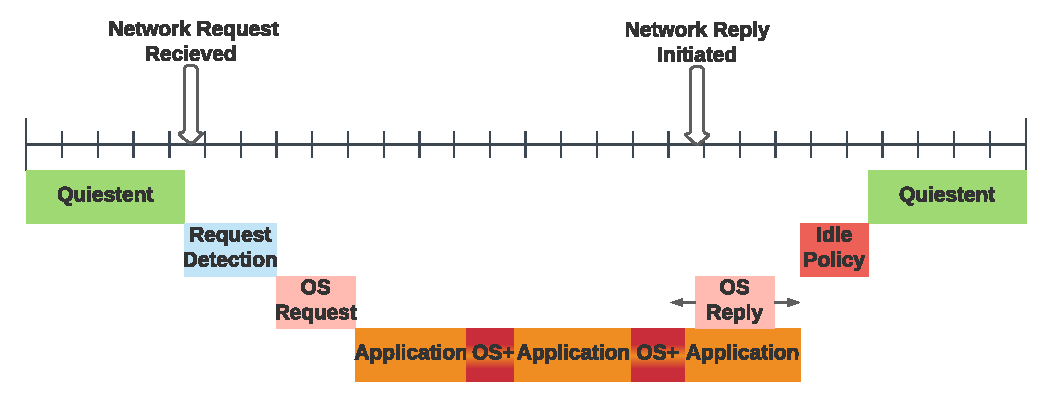
\includegraphics[width=1.1\columnwidth]{figures/timeline_chart}
\vspace*{-10mm}
\caption[]{Application processing request timeline.}
\label{fig:timeline}
\vspace{-0.20in}
\end{figure}

From an OS perspective we break down network driven processing into stages that allows us to organize and reflect the OS and application interaction with the workload request timeline. This break down is illustrated in figure~\ref{fig:timeline}\footnote{Although drawn from perspective of a single core, this path length is abstract enough to represent in multi-threaded applications and across modern network hardware}.
% TODO
% We believe the important aspects of OS/network loads are shown in figure 1
% abstraction 
% how we came up with this, to tease apart the interactions
%\textbf{TODO:General nature of the timeline graph across system and network hardware}  

\subsection{Quiescent}
\label{sec:workflow:Quiescent}
Given the packet and transactional nature of network driven services, a quiescent period, in which no requests are present at the server, precedes activity on the server. 

The nature of the workloads drive the length of quiescent period and of course the nature of the work required to service the request (the additional components of the diagram that will be discussed next).  Network services tends to fall into two broad categories Open and Closed Loop.   

\subsubsection{Open Loop:}
\label{sec:workflow:openloop}
In an open loop scenario like a Memcached workload, the external request rate induces an inter-arrival gap that will drive the quiescent period -- longer at lighter loads (lower queries per second (QPS)) and shorter at heavier loads (higher QPS). The arrival rate can largely be considered independent of the time required to service a request. Moreover, providers often set a Service-level Agreement (SLA) target, such as some percentage of requests to be completed under a stringent time budget. There have also been a wealth of research in using these SLA headrooms to lower datacenter energy use mainly by decreasing processor frequencies~\cite{Dynamo, SmoothOperator, oldi-pegasus, adrenaline, heracles, energyproportion, warehouse-power}.
% others have noted this is ripe to explore the trade-offs
%, therefore categorizing system performance into acceptable and unacceptable
%System performance is typically evaluated in terms of the 99\% tail latency it achieves.  
%such as a 99\% tail latency of 500${\mu}$s
%Many interesting interactions and trade-offs exist in Open Loop workloads to affect the latency below the SLA targets and the energy consumed. 

\subsubsection{Closed Loop:}
\label{sec:workflow:closed_loop}
Examples of closed loop workloads are snapshotting a database to a remote server, video streaming or a middle tier service within a data center~\cite{Barroso:2009:DCI:1643608, oldi-study, oldi-pegasus, warehouse-power, energyproportion, WebSearch}.  The work to be done is a sequence of requests that have an inter-dependency on each other. Specifically, the arrival of the next request depends on how fast it takes to service the current request. From a server's perspective, the quiescent period will be bounded by time to transmit both the request and the reply, as well as the time on the client to generate the next request.  
In the closed loop setting, one would like the server to complete every request quickly so that the overall time to complete a task is minimized. However, we find that depending on the nature of the workload and the quiescent period, composed of the network transmission times and client servicing time, there still exist interesting opportunities explore energy-performance trade-offs.
% polling in nodejs/netpipe - edp
% heavy computation vs light computation
% msg size differences
% itr delay -> edp

%However, the quiescent period is bounded by the network round trip time, that depends on  the size of a request and reply packets, and the remote processing time. System performance is largely evaluated on how fast a server can complete the entire task given a network link speed and a remote system.  Given workload specific characteristics such as the processing required and round-trip costs it is possible, as we will see, to find configurations in which the OS interacts with slowing down to improve both time and energy. 

%We know from previous research in energy proportionality in datacenters, the nature of web-centric applications causes diurnal troughs~\cite{Barroso:2009:DCI:1643608, oldi-study, oldi-pegasus, warehouse-power, energyproportion, WebSearch}, and one method with which to increase energy efficiency during these troughs is to increase performance. We find even in the performance driven closed loop applications, there still exist interesting trade-offs between OSes.

%Given our goal of studying and explaining the implications of the OS on network driven processing our analysis framework, and evaluation, includes closed loop settings.  In particular, we use a simple ping-pong application to stress OS behavior while varying packet-sizes to reveal how OS path length and path efficiency interacts with slowing down processing, relative to the round trip time observed at the server.  Additionally we use a second closed loop that stresses single core application processing with negligible packet sizes to evaluate if OS structure can impact the application efficiency.  

% Often research tends to categorize close loop settings as either not representative of cloud computing or imply that energy-performance tradeoffs are not interesting due to the hight utilization closed-loop processing can imply.  
\subsection{OS Request Detection}
Fundamental to any operating system is how it detects and schedules processing in response to IO device activity.  At the two extremes are interrupt and poll driven detection.  

\subsubsection{Interrupt driven IO}
\label{sec:workflow:interruptio}
Using interrupts has three important implications: 1) it can be used to wake a processor from a halted state, which the OS entered to sleep the processor (c-states), in response to external activity, 2) allow an OS to arbitrate processing across competitive devices in a multi-programmed/multi-device setting, 3) interrupts have inherent performance costs associated with it --  latency in starting to handle a request, either because of the costs associated with preempting work~\cite{whenpollisbetter} or c-state exit penalties\cite{cpuidle_policy}. Interrupts can also have a negative impact on the instruction efficiency, such as Instructions Per Cycle (IPC), due to induced micro-architecture hazards such as the inability to pre-fetch or speculatively execute across an interrupt.
%% brings in angle of energy and performance

\subsubsection{Poll driven IO}
%todo: modify to ack use of halt on cache line in stead of just polling.  
\label{sec:workflow:pollio}
Most modern NICs devices expose a cache-friendly interface that permits the processors to read a per-core memory address to determine if the device has received data that requires processing by the core.  This allows software to directly poll the device and initiate software handling without an interrupt.  This approach reduces latency and other performance penalties associated with interrupt driven IO but requires a busy CPU. In the extreme, a customized OS path supporting a single application can run a poll loop on every core to constantly check for work, conduct the work and then go back to polling for new work and thus never halting the processors \footnote{It is worth noting processors also have the ability to halt in a way that an update to a cache line will awaken it, there exists the possibility of implementing the poll in combination with sleep states. We do not explore this possibility, leaving it for future work.}.

%However, the period in which the device is checked requires CPU activity and thus limits the ability to halt the cores when there is no work to be done.

%Kim et al.\cite{pacingtoidle}, referred to a regime in which one keeps the processor busy as 'no-idle', an alternative energy management strategy. In the context of network driven processing we will refer to this as an aggressive polling or simply polling strategy.  In general, such an aggressive poll approach is assumed to maximize performance by avoiding interrupt overheads and minimize latency at a cost to increased energy use. 

\subsubsection{Hybrid driven IO}
\label{sec:workflow:hybridio}
% https://wiki.linuxfoundation.org/networking/napi
A general purpose OS typically exploits some form of hybrid IO strategy alternating between interrupts and polling when servicing high speed NICs. A common strategy is to use interrupts when the load is low and switch to polling when load is high and back to interrupts when load reduces.  A general purpose OS, even under sustained high load, bounds the poll phase to avoid the starving other devices and software. Linux's New API (NAPI)\cite{NAPI} framework implements this hybrid scheme.
%% these ideas help to explain the vertical of slowing down proceessor on Linux netpipe, memcached at really low QPS

%% Han - not sure we need to examine it in this detail, seems like re-explanation of the paragraph above, think NAPI and its implementation is already well known
%The first arrival of a packet generates an interrupt which switches the servicing of the device to polling if some threshold of packets are present.  If the number of packets drop below the threshold when the device is polled or a time limit for poll is exceeded the device will no longer be polled and interrupts re-enabled in order to detect activity on the NIC.  
%The NAPI framework, in addition to NIC processing budgets,  supports prioritization across devices. 
% In Linux the NAPI polls are processed via softirqs.  Checks for and processing of softirqs happens when ever the system returns to userspace or a hardware interrupt exits.

Specializing an OS to support the execution of a single application can explore more extreme strategies like the aggressive polling, described above, given that it need not arbitrate the device or cores and can be programmed and integrated with a single application.  
%% a general purpose must not starve out vs specialized os

\subsubsection{Interrupt Delaying}
\label{sec:workflow:itrdelay}
%\tikzstyle{startstop} = [rectangle, rounded corners, minimum width=3cm, minimum height=1cm,text centered, draw=black, fill=red!30]
\tikzstyle{io} = [trapezium, trapezium left angle=70, trapezium right angle=110, minimum width=3cm, minimum height=1cm, text centered, draw=black, fill=blue!30]
\tikzstyle{process} = [rectangle, minimum width=3cm, minimum height=1cm, text width=2cm, text centered, draw=black, fill=orange!30]
\tikzstyle{decision} = [diamond, minimum width=3cm, minimum height=1cm, text width=1cm, text centered, draw=black, fill=green!30]
\tikzstyle{arrow} = [thick,->,>=stealth]

%\begin{figure}
\centering
%\resizebox{5cm}{3cm}{%
\begin{tikzpicture}[node distance=2cm]

\node (start) [startstop] {ITR=\textit{n} $\mu$s};
\node (dec1) [decision, below of=start] {ITR==\textit{0}?};
\node (pro1) [process, right of=dec1, xshift=1.5cm] {ITR-=\textit{2} $\mu$s};
\node (dec2) [decision, below of=dec1, yshift=-0.5cm] {RX/TX Event?};
\node (pro2) [startstop, left of=dec2, yshift=1.5cm, xshift=-0.8cm] {Assert Interrupt};

\draw [arrow] (start) -- node[anchor=west] {check} (dec1);
\draw [arrow] (dec1) -- node[anchor=north] {no} (pro1);
\draw [arrow] (pro1) |- node[anchor=west] {update} (start);
\draw [arrow] (dec1) -- node[anchor=west] {yes} (dec2);
\draw [arrow] (dec2) edge[loop right]node{no} (dec2);
\draw [arrow] (dec2) -- node[anchor=east] {yes} (pro2);
%\draw [arrow] (pro2) -| node {} (start);
\draw [arrow] (pro2) |- node[anchor=east] {reset} (start);
\end{tikzpicture}
%}
%\vspace*{-5mm}
%\caption{ITR-Delay algorithm flowchart.}
%\label{fig:itr_delay_flowchart}
%\vspace{-.25in}
%\end{figure}
%We flowchart the algorithm from the NIC's datasheet~\cite{82599} in  Figure~\ref{fig:itr_delay_flowchart}
A common feature of modern high speed NICs is the ability to delay the delivery of interrupt when an event such as packet arrival or transmission completion. By manipulating this setting, software can limit the minimum time between interrupts or in other words the maximum rate at which the NIC events can interrupt the CPUs. The NIC used in this study exposes this mechanism via an Interrupt Throttling (ITR) setting. Software uses the ITR register to configure a delay in 2$\mu$s increments.  If the spacing of events, such as packet reception, is less than  $2{\mu}s \times ITR$ the NIC will delay assertion.  If on the other hand events are sufficiently separated an interrupt will be asserted immediately.   

By default the Linux device driver attempts to automatically set this interrupt delay value to reduce interrupt overheads.  We disable this feature and manually control its value to explore the impact of delaying interrupts on performance and energy. Delaying interrupt detection introduces an OS control that can interact with energy and performance. For example, delaying a interrupt can induce prolonged quiescence periods, in which processor idle policies can take advantage of.

%Combining interrupt driven IO and delaying interrupt assertion via ITR setting, we can explore the impact of delaying packet detection and thus delaying processing of requests.

  %Depending of the state of the processor the NIC can buffer packets in its own memory or on the main memory of the host\footnote{According to the data sheet if the processor is in sleep state packets can only be buffered on the card's limited memory and once exhausted packets will be dropped}.  

%% TODO: may move down

\subsection{OS Request Processing}
\label{sec:workflow:osreqproc}

Once the OS detection mechanism identifies that the NIC has data to process, several components of OS functionality must be run in accordance with the execution model of the OS. Specifically, the OS's network stack parses the received packet's layer 2 frames, TCP/IP headers and eventually to the application layer for processing. %% TODO shorten

%%Specifically, device driver code must dequeue layer 2 frames and schedule them for processing by the appropriate network protocol code. This code must ultimately determine the application end point, a port in the case of IP and TCP, and enqueue, the encapsulated data, for application processing. 

This work on a general purpose OS, is typically split between two levels of scheduling; 1) interrupt level in which minimal work is done but at the highest critical priority and is run to completion (typically called the top-half processing), 2) the so-called bottom-half uses various kernel facilities to execute both device driver logic and protocol processing in a manner that can be preempted and rate limited.  Regardless, all this work is done at the OS privilege domain and ultimately prepares data for the workload specific pre-emptable application processing which is independently scheduled at lower privilege and priority. %% contrasted with specialized os

Library operating systems that are customized for a specific application and processing model often shed much of the above complexity both shortening the path and eliminating the above privilege scheduling domains\cite{10.1145/2997641,10.1145/2812806,EbbRT}.  Rather, they can exploit short-cuts that allow run to completion execution of all the logic, including application processing in response to detecting device activity.  As such, we can use the library OS to explore the impacts of shorter and OS hot-paths customized to running a single network service.  

\subsubsection{Application Processing}
\label{sec:workflow:appproc}

Once the OS has completed protocol processing it enables application logic to begin.  Depending on the workload this may be very simple as in the case of a workload like memcached or it require significant cpu activity as in the case of  an application server written in managed runtime such as nodejs or one that does non-trivial computational work to service a request. 

As illustrated, during application processing the OS logic may be interleaved.  This work roughly falls into two categories, synchronous work done in service of this application request (page-faults, system calls, etc) and asynchronous work not having to do with this request (OS background work, processing of other requests or processes).

Library OS's can often avoid interleaving asynchronous work, unrelated to the request handling,  and thus minimize jitter and improve IPC. %% application work is fixed typically

\subsubsection{OS Reply Processing}
\label{sec:workflow:osrepproc}

Figure~\ref{fig:timeline} shows that at some point during application processing a reply is generated and submitted to the OS for transmission.  This can often be handled in an asynchronous fashion depending on the OS semantics.  Where the OS can initiate protocol processing and device transmission in parallel with the remaining application request processing logic (eg. book keeping, cleanup and preparation for the next request).

This potential overlap is an important distinction as it reveals that some applications may have an associated opportunity for a performance/energy optimization.  Specifically, it is possible given a particular arrival rate that there maybe ways of slowing down that permit the remaining application work to overlap with the time for the next request to arrive in both a closed and open loop settings.  As such it maybe possible that trade-offs in sleep state latency, interrupt overheads and polling leads to better performance at lower energy consumption.  

\subsubsection{Idle Policy}
\label{sec:workflow:idlepolicy}

If all processing is complete, no traffic is pending and aggressive polling is not in use the OS can enact a policy that select a hardware sleep state (C-State) to halt the core to.  The sleep states and various policies has been extensively studied\cite{dynsleep,dreamweaver,slowdownorsleep}.  Each sleep state is has an associated reduction in static power consumption. In the extreme, the deepest sleep states can flush micro-architectural state such as caches and power down these structures. However, each sleep state also imposes a progressively larger wake-up latency and potential impact on execution efficiency given the possible flushing of state~\cite{7425206}. %See \cite{brooks,udpm} for more information regarding C-States. 

%If there is space we might want to add the c-state for our processor similar to what was done in Brooks

There is clearly a relationship between the Idle Policy and Request Detection processing.  For a general purpose OS the normative assumption is both are interrupt driven.  Where an inter-dependency between the halt and interrupt mechanisms of the processor is exploited.  

In our study we allow Linux's scheduler and default idle driver to decide if a core should be halted and to what state.  The software exploits various statistics to estimate how long the core is likely to be idle. It takes into account an estimate of when the next interrupt will likely occur from any source.  This is a subtle implementation that interacts across many layers of the OS software including the device drivers.  The idle driver framework also includes code provided by the processor manufacturer to evaluate the latency penalties and suggested minimum residency times.  This allows us to see the impacts of making informed decisions regarding sleep states.  

We use the Library OS to two simple policies.  In the first, when there is no work to process on a core we simply put the processor into the deepest sleep state (C7), thus ignoring any trade-offs in use of other sleep states.   This allows us to focus on the interaction that slowing down the processor and adjusting the ITR can have with the fixed use of a deep sleep.   The second approach we take is the aggressive pool configuration, as discussed above, where we have no idle policy and simply immediately go back to using poll to implement request detection.
%% discussion section later about alternatve sleep state policies